\documentclass[12pt,a4paper,openany,twoside]{report}

\usepackage[utf8]{inputenc}
\usepackage[italian]{babel}
\usepackage{fancyhdr}
\usepackage{indentfirst}
\usepackage{graphicx}
\usepackage{newlfont}
\usepackage{amssymb}
\usepackage{amsmath}
\usepackage{latexsym}
\usepackage{amsthm}
\usepackage{listings}
\usepackage[hyphens]{url}
\usepackage{hyperref}
\usepackage[square,numbers,sort]{natbib} % Gestione bibliografia richiesta
\usepackage{xcolor}
\usepackage{minted}
\usepackage{tabularx}
\usepackage{makecell}
\usepackage{geometry}
\usepackage{acronym}
\usepackage{subcaption}
\usepackage{float}
\usepackage{csquotes}
\usepackage{todonotes}

\bibliographystyle{unsrtnat} % Stile bibliografia
\lstset{frame=single,breaklines=true}
\setcounter{secnumdepth}{4}
\setcounter{tocdepth}{4}
\oddsidemargin=30pt
\evensidemargin=20pt
\linespread{1.3}
\graphicspath{{./figures/}{./img/}} % Cartelle immagini

% Header e Footer
\pagestyle{fancy}\addtolength{\headwidth}{20pt}
\renewcommand{\chaptermark}[1]{\markboth{\thechapter.\ #1}{}}
\renewcommand{\sectionmark}[1]{\markright{\thesection \ #1}{}}
\rhead[\fancyplain{}{\bfseries\leftmark}]{\fancyplain{}{\bfseries\thepage}}
\cfoot{}

% --- COMANDI UTILI ---
\newcommand{\nchapter}[1]{
  \clearpage{\pagestyle{empty}}
  \chapter{#1}
  \lhead[\fancyplain{}{\bfseries\thepage}]{\fancyplain{}{\bfseries\rightmark}}
}
\newcommand{\unchapter}[1]{
  \clearpage{\pagestyle{empty}}
  \chapter*{#1}
  \rhead[\fancyplain{}{\bfseries #1}]{\fancyplain{}{\bfseries\thepage}}
  \lhead[\fancyplain{}{\bfseries\thepage}]{\fancyplain{}{\bfseries #1}}
  \addcontentsline{toc}{chapter}{#1}
}
\newcommand{\unsection}[1]{\section*{#1}\addcontentsline{toc}{section}{#1}}

% --- ACRONIMI ---
\acrodef{IoT}{Internet of Things}
\acrodef{API}{Application Programming Interface}
\acrodef{BaaS}{Backend as a Service}

\begin{document}

% 1. Frontespizio
\begin{titlepage}

\newgeometry{
  left=20mm,
  right=20mm,
  top=20mm,
  bottom=20mm
}

\begin{center}

\includegraphics[width=6.5cm,height=4.7cm]{../figures/unibo_icons/marchio-di-ateneo.png}

\vspace{10mm}

DIPARTIMENTO DI INFORMATICA - SCIENZA E INGEGNERIA\\
Corso di Laurea Triennale in Ingegneria e Scienze Informatiche

\vfill
\vspace{15mm}

{\Large{\textbf{EcoSpot: Un'App Mobile per la Valorizzazione della Biodiversità del Parco del Delta del Po Tramite Gamification e Dati Ambientali
}}}

\vspace{15mm}
\vfill

\textit{Elaborato in}\\
\textbf{Programmazione di Sistemi Mobile}

\end{center}

\vspace{15mm}

\par
\noindent
\begin{minipage}[t]{0.4\textwidth}{
  \textit{Relatore}\\
  \textbf{Prof. Catia Prandi}

  \vspace{5mm}
  
  \textit{Correlatore}\\
  \textbf{Dott. Gianni Tumedei}
}\end{minipage}
\hfill
\begin{minipage}[t]{0.4\textwidth}\raggedleft{
  \textit{Presentata da}\\
  \textbf{Alex Frisoni}
}\end{minipage}

\vspace{15mm}

\begin{center}
\rule[2mm]{\textwidth}{0.4mm}

\large{\textbf{
Sessione di Marzo 2026\\
Anno Accademico 2025/2026
}}
\end{center}

\end{titlepage}


\pagenumbering{roman}

% 2. Abstract/Introduzione
\unchapter{Introduzione}
\addcontentsline{toc}{chapter}{Introduzione}
\markboth{Introduzione}{Introduzione}

Il Parco del Delta del Po costituisce uno degli ecosistemi più complessi e delicati del panorama europeo, 
rappresentando una Riserva di Biosfera MAB UNESCO di inestimabile valore naturalistico. 
Focalizzando l'attenzione in particolare sul versante emiliano-romagnolo, il Parco offre un 
mosaico paesaggistico unico che spazia dalle vaste zone umide delle Valli di Comacchio e dalle antiche 
Saline di Cervia, fino alle fitte foreste del Bosco della Mesola e alle storiche pinete costiere. 
Questa straordinaria varietà di habitat lagunari, fluviali e boschivi lo rende una meta d'eccellenza per il turismo sostenibile e un rifugio 
vitale per innumerevoli specie animali. L'avifauna rappresenta senza dubbio una delle ricchezze più celebri del territorio, che ospita eleganti 
colonie di fenicotteri rosa, oltre a specie caratteristiche e protette come l'avocetta, il cavaliere d'Italia, 
il cormorano e il falco di palude.

Tuttavia, la fragilità di questo ecosistema e la sopravvivenza dei volatili sono oggi messe a dura prova dai mutamenti climatici e dalle alterazioni idrogeologiche. 
Tra i fenomeni più critici e insidiosi spicca l'intrusione del cuneo salino, ovvero la progressiva risalita delle acque marine all'interno degli alvei fluviali del delta e 
nelle falde acquifere sotterranee. Tale dinamica, innescata e aggravata dai prolungati periodi di siccità, dalla drastica riduzione della portata d'acqua dolce dei fiumi 
e dal fenomeno della subsidenza, altera profondamente il delicato equilibrio tra acqua dolce e salmastra. Questo sbilanciamento degrada rapidamente le aree di 
nidificazione e di foraggiamento, minacciando direttamente la fauna e la flora, oltre a rischiare di compromettere irrimediabilmente le attività agricole del territorio limitrofo.

In questo scenario di vulnerabilità, dove la tutela della biodiversità aviaria diventa un'emergenza prioritaria, l'osservazione passiva 
non è più sufficiente; si rende necessario un monitoraggio scientifico costante e capillare. In questa cornice si inserisce il progetto DISCOV.ER, 
un'iniziativa avanzata di ricerca e innovazione tecnologica mirata alla creazione di un Digital Twin dell'ecosistema del Delta del Po. 
Il progetto si avvale di una vasta rete di sensori \ac{IoT} immersi direttamente nei corpi idrici e dislocati in punti strategici. Questi dispositivi sono programmati per rilevare e 
trasmettere in tempo reale dati ambientali, tra cui i livelli di salinità dell'acqua, le variazioni di temperatura, la conducibilità, 
la velocità del vento e ulteriori parametri di rilievo.

La disponibilità di questa mole di dati richiede però strumenti digitali adeguati affinché possa essere resa 
facilmente accessibile e consultabile anche dal grande pubblico. 
Dati invisibili come quelli sul cuneo salino nascondono infatti impatti devastanti sulla sopravvivenza degli animali. 
È proprio da questa necessità di 
tutelare il patrimonio faunistico e dare voce all'ecosistema che nasce \textit{EcoSpot}, un'applicazione 
mobile sviluppata all'interno del progetto DISCOV.ER e concepita per fungere da ponte tra la complessa 
dimensione tecnologica di monitoraggio e l'esperienza naturalistica del visitatore. L'app offre la possibilità di visionare 
le metriche dei sensori \ac{IoT} sulla mappa in modo chiaro e di immediata comprensione. 
Rendendo tangibile l'impatto dei cambiamenti ambientali sugli habitat e sulle specie che li popolano, l'applicazione 
informa l'utente e lo rende pienamente consapevole dell'ecosistema che sta attraversando.

La parte centrale di EcoSpot, tuttavia, risiede nell'obiettivo finale di questa consapevolezza: la salvaguardia attiva della fauna. 
Per incentivare questo principio l'applicazione integra meccaniche di gamification e sfide interattive studiate per incentivare 
un'esplorazione responsabile e rispettosa del territorio.
Attraverso il completamento delle sfide proposte, il visitatore viene attivamente coinvolto, sviluppando una maggiore propensione al rispetto e alla tutela dell'ecosistema.
EcoSpot non si limita dunque alla funzione di guida turistica, ma si configura come una piattaforma educativa avanzata che sfrutta l'infrastruttura di DISCOV.ER 
per connettere in modo bidirezionale la realtà fisica del Parco alla sua rappresentazione digitale.

Il presente lavoro documenta l'intero processo di realizzazione dell'applicazione, seguendo un percorso logico che parte dall'analisi del contesto 
per giungere alla soluzione ingegneristica finale.
L'analisi si apre con il primo capitolo, inquadrando lo scenario territoriale di riferimento. 
Attraverso l'esame delle peculiarità idrogeologiche e faunistiche dell'area, con un focus centrale sulla tutela dell'avifauna, si osserva l'evoluzione 
dell'offerta turistica verso modelli di fruizione intelligente del patrimonio. 
In questo quadro vengono approfonditi i paradigmi abilitanti quali il monitoraggio collaborativo e l'uso di elementi motivazionali per 
incentivare comportamenti responsabili. Tale studio preliminare si conclude posizionando l'app come uno strumento innovativo per 
la divulgazione e il coinvolgimento attivo del visitatore.

Sulla base di queste premesse, si sviluppa il secondo capitolo, che si apre con l'analisi dei requisiti funzionali e non funzionali, 
per poi passare alla vera e propria fase di progettazione. 
A fronte delle necessità emerse, vengono motivate le scelte architetturali adottate: da un lato l'utilizzo del framework Flutter per uno 
sviluppo multipiattaforma capace di garantire un'esperienza fluida su vari sistemi operativi; dall'altro la scelta della suite Google Firebase 
come infrastruttura di backend, ideale per gestire autenticazione e dati in tempo reale con un'elevata scalabilità.

Infine, nell'ultimo capitolo la tesi illustra nel dettaglio l'implementazione tecnica dell'applicativo, approfondendo 
l'architettura gestita tramite Riverpod, essenziale per assicurare una gestione dello stato dell'interfaccia solida e manutenibile. 
Vengono inoltre esposte le logiche impiegate per la mappa interattiva e l'integrazione a livello di codice dei flussi di dati provenienti dai sensori IoT, 
mostrando in che modo siano stati tradotti in funzionalità concrete. 

Lo studio si conclude con le considerazioni finali sul lavoro svolto e una riflessione sugli sviluppi futuri, 
ipotizzando come l'integrazione di tecnologie quali l'intelligenza artificiale e la realtà aumentata possa ulteriormente potenziare 
l'impatto di EcoSpot sulla salvaguardia del patrimonio faunistico.

\tableofcontents

\clearpage{\pagestyle{empty}}
\pagenumbering{arabic}

% Capitoli
% !TEX root = ../thesis-main.tex
\chapter{Inquadramento territoriale e scenario di riferimento}
\label{chap:context}

\section{La Riserva di Biosfera MAB UNESCO: un ecosistema da valorizzare}
Il Parco del Delta del Po costituisce la più vasta zona umida d’Italia e una delle aree europee a più alta biodiversità, grazie al mosaico di lagune salmastre, valli da pesca, canneti, pinete costiere, dune e zone agricole. Questa varietà di habitat sostiene un numero elevatissimo di specie vegetali e animali, motivo per cui l’area è riconosciuta come Riserva di Biosfera MAB UNESCO \cite{unesco_po_official} \cite{biosfera_mab_reason}. Dal punto di vista faunistico, il Delta ospita oltre 300–350 specie di uccelli tra nidificanti, svernanti e migratori, rendendolo uno dei siti più importanti d’Europa per l’avifauna acquatica. Tra le specie più caratteristiche figurano i fenicotteri rosa (Phoenicopterus roseus), divenuti simbolo del paesaggio lagunare, insieme ad aironi cenerini, cormorani, cavalieri d’Italia, avocette, falchi di palude e molte altre specie legate alle zone umide. I fenicotteri sfruttano le acque basse e salmastre delle valli e delle lagune per alimentarsi, formando spesso grandi concentrazioni di individui che possono raggiungere diverse migliaia di esemplari nei periodi di maggior presenza. Questa specie è considerata particolarmente protetta a livello internazionale ed è indicativa di buone condizioni ecologiche degli ambienti umidi costieri. Accanto all’avifauna, il Parco ospita una ricca fauna ittica (circa 60 specie, alcune tipiche del Delta), numerosi invertebrati legati alle acque e ai sedimenti, e una flora dominata da canneti, flora adattata agli ambienti salmastri e ultimi lembi delle antiche foreste di pianura , che contribuiscono a funzioni ecosistemiche chiave come depurazione delle acque, protezione costiera e stoccaggio di carbonio. L’insieme di questi elementi fa del Delta del Po un laboratorio naturale per lo studio e la gestione della biodiversità lagunare in un contesto in cui conservazione e attività umane (agricoltura, pesca, turismo) devono coesistere in modo sostenibile.

\subsection{Biodiversità e patrimonio naturalistico lagunare}
L'area è un habitat cruciale per numerose specie, tra cui il Fenicottero Rosa (\textit{Phoenicopterus roseus}), simbolo della biodiversità locale. La flora comprende specie alofile come la Salicornia, adattate agli ambienti salmastri tipici delle lagune costiere.

\subsection{Specificità idro-morfologiche del versante emiliano-romagnolo}

\paragraph{Il relitto forestale della Mesola}
Riserva naturale orientata, rappresenta l'ultimo residuo delle antiche foreste termofile litoranee che un tempo ricoprivano la costa adriatica.

\paragraph{Il sistema delle Valli di Comacchio}
Un complesso di lagune salmastre dove la gestione idraulica è fondamentale. È qui che il progetto EcoTwin concentra parte del monitoraggio, in particolare nelle stazioni di Bellocchio e Foce, aree strategiche per l'avifauna \cite{parcodelta}.

\paragraph{La pressione antropica sulla fascia costiera}
Aree soggette a forte pressione antropica, che necessitano di strumenti innovativi per veicolare i flussi turistici verso forme di fruizione più sostenibili e consapevoli.

\subsection{Evoluzione della domanda turistica verso la fruizione consapevole}
I visitatori moderni richiedono informazioni puntuali e in tempo reale. Nell'ottica dello \textit{Smart Tourism} \cite{smart_tourism}, non è sufficiente indicare i punti di interesse statici; è necessario fornire dati contestuali sulle condizioni ambientali (es. livelli dell'acqua, meteo specifico) per pianificare l'escursione in sicurezza.

\section{Paradigmi tecnologici per la gestione delle aree protette}

\subsection{Sistemi di geolocalizzazione e mappatura dinamica}
Le mappe digitali hanno progressivamente sostituito quelle cartacee, permettendo la geolocalizzazione dinamica dell'utente e l'interazione con i Punti di Interesse (POI) distribuiti sul territorio.

\subsection{Il monitoraggio partecipativo attraverso la Citizen Science}
Il coinvolgimento dei cittadini nella raccolta dati, noto come \textit{Citizen Science} \cite{citizen_science}, trasforma il turista da osservatore passivo a partecipante attivo nel monitoraggio della biodiversità, contribuendo alla ricerca scientifica.

\subsection{Meccaniche ludiche per l'incentivazione territoriale}
La \textit{Gamification} è definita come l'uso di elementi di game design in contesti non ludici \cite{gamification_def}. Nel progetto EcoTwin, meccaniche quali punti esperienza (XP), livelli e badge (es. "Leggenda del Delta") vengono impiegate per incentivare l'esplorazione fisica di nuovi habitat.

\section{Caso di studio: l'ecosistema digitale EcoTwin}

\subsection{La sintesi tra dati ambientali ed esperienza utente}
L'obiettivo principale è la creazione di un "Digital Twin" \cite{digital_twin_env} informativo che colleghi i dati oggettivi dei sensori idrografici (livello canali, salinità) all'esperienza soggettiva del visitatore.

\subsection{Architettura del sistema e integrazione IoT}
L'architettura proposta si basa su un'applicazione mobile sviluppata in Flutter \cite{flutter}, collegata a un backend Cloud per la sincronizzazione dei progressi e a un'infrastruttura IoT per l'acquisizione dei dati ambientali in tempo reale.

\subsection{Impatto atteso sull'engagement e sulla consapevolezza ecologica}
Si attende un aumento dell'engagement dei visitatori e una maggiore consapevolezza ecologica, dimostrando come le tecnologie digitali possano supportare efficacemente la gestione e la fruizione delle aree protette.
%!TEX root = ../thesis-main.tex
\chapter{Tecnologie e Progettazione}
\label{chap:technologies}

Questo capitolo presenta l'analisi degli obiettivi e la progettazione del sistema EcoSpot, descrivendo l'architettura logica e le scelte tecnologiche adottate per lo sviluppo dell'applicazione mobile e la sua integrazione con i servizi cloud e IoT.


\section{Obiettivi del progetto}
\label{sec:project_goals}

La progettazione di EcoSpot è guidata da quattro obiettivi strategici, volti a coniugare l'esperienza turistica con la consapevolezza ecologica e le moderne tecnologie mobili.

\begin{itemize}
    \item \textbf{Divulgazione e Citizen Science:} l'obiettivo è diffondere la conoscenza della biodiversità locale attraverso una \textit{collezione digitale} strutturata e partecipativa. L'applicazione non si limita a offrire un catalogo dettagliato di specie (suddivise in categorie come uccelli, mammiferi, pesci e aree verdi), ma abilita pratiche di \textit{Citizen Science}: gli utenti possono contribuire attivamente al monitoraggio del territorio inviando segnalazioni georeferenziate e fotografiche, trasformando la semplice osservazione in un percorso di tutela condivisa.

    \item \textbf{Incentivazione del turismo lento:} il sistema mira a favorire un'esplorazione rispettosa del territorio sfruttando meccaniche \textit{location-based}. Grazie alla geolocalizzazione e al \textit{geofencing}, l'utente è incentivato a raggiungere fisicamente luoghi reali (valli, argini, punti di osservazione) per sbloccare i contenuti e validare le scoperte, promuovendo così una mobilità dolce e un presidio attivo degli habitat, in contrapposizione al turismo di massa.

    \item \textbf{Monitoraggio ambientale integrato:} il progetto intende rendere accessibili parametri ecologici complessi tramite l'aggregazione di dati IoT in tempo reale. L'app si interfaccia con le API di enti territoriali (es. progetto DISCOV.ER) per i dati idrografici (livello, temperatura, conducibilità) e integra servizi meteorologici come Open-Meteo \cite{open_meteo_api}, rendendo visibili all'utente fattori invisibili ma vitali per l'ecosistema lagunare.

    \item \textbf{Incremento del coinvolgimento (Gamification):} l'ultimo obiettivo è massimizzare la ritenzione e la partecipazione dell'utente attraverso la \textit{gamification}. L'uso di elementi ludici come punti esperienza (XP) e livelli dinamici (da ``Esploratore'' a ``Leggenda del Delta'') serve a rafforzare il senso di appartenenza al territorio e a stimolare comportamenti virtuosi, premiando l'interazione fisica con il Parco.
\end{itemize}

L'integrazione di questi quattro pilastri mira ad aumentare l'attenzione dei visitatori, offrendo un'esperienza che combina contenuti informativi, esplorazione fisica e feedback immediati sulle pratiche sostenibili. Al tempo stesso, la possibilità di accedere a dati ambientali in tempo quasi reale e di collegarli alle osservazioni sul campo contribuisce a sviluppare una maggiore consapevolezza ecologica, mostrando in modo concreto la fragilità e il valore degli ecosistemi lagunari. In questo senso, EcoSpot si configura non solo come strumento di guida turistica, ma come piattaforma di educazione ambientale e di supporto alla gestione sostenibile delle aree protette del Delta del Po.

\section{Analisi dei Requisiti}
\label{sec:requirements}

La fase di progettazione è stata preceduta da un'analisi dettagliata dei requisiti, volta a definire il perimetro funzionale e le caratteristiche qualitative del sistema EcoSpot.

\subsection{Requisiti Funzionali}
I requisiti funzionali descrivono le interazioni specifiche tra l'utente e il sistema e definiscono le necessità informative della base di dati. Sulla base degli obiettivi di progetto e dei casi d'uso identificati, sono stati definiti i seguenti requisiti:

\begin{enumerate}
    \item \textbf{Mappa Interattiva} \label{req:mappa}
    Il sistema deve fornire una mappa digitale del Delta del Po che visualizzi i layer informativi relativi alle aree di interesse naturalistico (flora e fauna) e alle stazioni di monitoraggio ambientale. La mappa deve supportare l'interazione touch (pan e zoom) e adattare la densità delle informazioni in base al livello di zoom.

    \item \textbf{Posizione in Tempo Reale} \label{req:tracking}
    L'applicazione deve acquisire e monitorare costantemente la posizione geografica dell'utente tramite GPS. Il tracciamento deve avvenire in background (ove permesso) o in foreground per garantire che la posizione sulla mappa sia sempre sincronizzata con lo spostamento fisico dell'utente.
    
    \item \textbf{Rilevamento di Prossimità} \label{req:geofencing}
    Per supportare la meccanica del "Turismo Lento", il sistema deve calcolare in tempo reale la distanza euclidea tra le 
    coordinate dell'utente e gli habitat o le aree verdi. Al raggiungimento di una soglia di tolleranza 
    specifica (definita come \textit{raggio di scoperta}, variabile tra 450 metri per la fauna e 800 metri per la flora), 
    il sistema deve innescare l'evento di "scoperta".
    
    \item \textbf{Profilo Utente} \label{req:profilo}
    Il database deve mantenere un profilo utente persistente e sincronizzato su cloud per gli utenti registrati, 
    memorizzando dati anagrafici e preferenze. Il sistema deve altresì supportare una modalità "Ospite" con persistenza 
    locale temporanea.
    
    \item \textbf{Sistema di Gamification} \label{req:gamification}
    Il sistema deve gestire la logica di progressione dell'utente. Ogni evento di scoperta deve assegnare una ricompensa in Punti Esperienza (XP), aggiornare l'inventario delle specie collezionate (sbloccando le relative schede informative) e ricalcolare il rango e il livello utente in base alle soglie predefinite.

    \item \textbf{Ricerca} \label{req:ricerca}
    Data l'elevata densità di elementi sulla mappa, il sistema deve fornire una barra di ricerca testuale per le specie e le aree verdi. 
    Questi strumenti devono permettere all'utente di ridurre la complessità visiva e isolare rapidamente i dati di interesse.

    \item \textbf{Dati Ambientali} \label{req:iot}
    Il sistema deve ingerire e visualizzare dati provenienti da fonti esterne eterogenee (stazioni \ac{IoT}). Il modello dati deve prevedere strutture flessibili per normalizzare letture di temperatura, livello idrometrico e conducibilità, rendendole consultabili in tempo quasi reale attraverso i marker sulla mappa.

    \item \textbf{Segnalazione} \label{req:segnalazioni}
    Gli utenti autenticati devono poter inviare segnalazioni georeferenziate. Ogni record deve comprendere una descrizione 
    testuale, la posizione GPS esatta (\texttt{GeoPoint}) e il timestamp di creazione. Le prove fotografiche devono essere 
    caricate su uno storage remoto (\textit{Cloud Storage}).

    \item \textbf{Progressione} \label{req:integrita}
    Per incentivare l'uso continuativo e garantire la coerenza dei dati, ogni modifica allo stato del giocatore (scoperta, level-up) deve essere gestita tramite transazioni atomiche. Questo impedisce condizioni di gara (race conditions) e duplicazioni di XP, assicurando che l'aggiornamento del livello e dell'inventario avvengano come un'operazione indivisibile.

    \item \textbf{Funzionamento Offline e Sincronizzazione} \label{req:offline}
    Considerata la potenziale assenza di copertura di rete in alcune aree del parco, il sistema deve garantire la fruibilità dei contenuti statici (schede informative) e della mappa (tramite caching) anche in modalità offline. Le azioni critiche dell'utente, come lo sblocco di una specie o l'invio di una segnalazione, devono essere memorizzate localmente in una coda di persistenza e sincronizzate automaticamente con il server remoto non appena la connettività viene ripristinata.

    \item \textbf{Compatibilità Multi-Piattaforma} \label{req:multipiattaforma}
    Il sistema deve essere sviluppato garantendo la piena compatibilità funzionale e visiva sia con il sistema operativo 
    Android che con iOS. L'interfaccia utente deve adattarsi alle linee guida specifiche delle piattaforme pur mantenendo un 
    design system coerente (Material Design 3) \ref{material_design_3}.
\end{enumerate}
\subsection{Requisiti Non Funzionali}
I requisiti non funzionali definiscono gli attributi di qualità del sistema, imponendo vincoli architetturali e prestazionali necessari per garantire un'esperienza utente soddisfacente, specialmente in un contesto di utilizzo in mobilità e all'aperto (\textit{outdoor}).

\begin{enumerate}
    \item \textbf{Usabilità e Accessibilità} \label{rnf:usabilita}
    L'interfaccia utente deve garantire la massima leggibilità anche in condizioni di forte illuminazione solare diretta, tipica delle escursioni diurne. Il sistema deve supportare il passaggio dinamico (o automatico) tra tema chiaro e scuro per mantenere un contrasto ottimale. Gli elementi interattivi (bottoni, card) devono rispettare le dimensioni minime di tocco (48x48dp) per facilitare l'uso in movimento.

    \item \textbf{Prestazioni e Reattività} \label{rnf:performance}
    Il rendering della mappa e delle animazioni di transizione deve mantenere un frame rate stabile di almeno 60 fps (fotogrammi al secondo) per evitare scatti (\textit{jank}) che comprometterebbero l'esperienza utente. Il tempo di avvio dell'applicazione (Cold Start) non deve superare i 2 secondi su dispositivi di fascia media.

    \item \textbf{Efficienza Energetica} \label{rnf:energia}
    Dato l'uso prolungato durante le escursioni e l'assenza di punti di ricarica nelle aree naturali, il consumo della batteria deve essere minimizzato. Il servizio di localizzazione deve adottare strategie di campionamento adattivo (es. riducendo la frequenza di aggiornamento GPS quando l'utente è fermo) per non drenare eccessivamente le risorse del dispositivo.

    \item \textbf{Manutenibilità del Codice} \label{rnf:manutenibilita}
    Il codice sorgente deve seguire i principi della \textit{Clean Architecture}, garantendo una netta separazione tra logica di business, interfaccia utente e gestione dei dati. L'adozione di standard di formattazione coerenti e la documentazione del codice devono facilitare le operazioni di debug e l'aggiornamento futuro del software da parte di altri sviluppatori.

    \item \textbf{Estensibilità e Scalabilità} \label{rnf:estensibilita}
    L'architettura del sistema deve essere progettata per accogliere future evoluzioni senza richiedere la riscrittura dei moduli principali. Deve essere possibile aggiungere nuove categorie di specie, nuovi layer cartografici o funzionalità di gamification aggiuntive (es. classifiche globali) attraverso l'estensione delle classi esistenti o l'integrazione di nuovi plugin.

    \item \textbf{Privacy e Sicurezza dei Dati} \label{rnf:privacy}
    Trattando dati sensibili relativi alla posizione geografica degli utenti, il sistema deve garantire la conformità con le normative vigenti (GDPR). I dati di localizzazione non devono essere condivisi con terze parti non autorizzate e, dove possibile, devono essere anonimizzati per le analisi statistiche aggregate.
\end{enumerate}
\section{Tecnologie}
\label{sec:technologies}

\subsection{Flutter e Dart}
Per lo sviluppo dell'applicazione EcoSpot è stato selezionato \textbf{Flutter} \cite{flutter}, il framework open-source sviluppato da Google che consente la realizzazione di applicazioni multipiattaforma native.
Questa scelta architetturale è stata motivata da diversi fattori strategici che rispondono agli obiettivi del progetto:

\begin{itemize}
    \item \textbf{Efficienza nello sviluppo (Single Codebase):} Flutter permette di gestire un'unica base di codice per Android e iOS. Questo ha ridotto drasticamente i tempi di implementazione, garantendo al contempo una parità di funzionalità tra le piattaforme senza la necessità di mantenere due team di sviluppo distinti.

    \item \textbf{Prestazioni grafiche (Impeller):} A differenza di altri framework ibridi, Flutter non utilizza webview ma un motore di rendering proprietario. Per EcoSpot è stato sfruttato il moderno motore \textbf{Impeller}, che sostituisce il precedente Skia. Impeller risolve i problemi di \textit{jank} (scatti) dovuti alla compilazione degli shader a runtime, pre-compilandoli e sfruttando le API di basso livello (Metal su iOS e Vulkan su Android). Ciò garantisce animazioni fluide a 60 FPS, fondamentali per la gestione delle mappe interattive e delle transizioni nelle schede delle specie.

    \item \textbf{Produttività (Hot Reload):} La funzionalità di \textit{Stateful Hot Reload} ha permesso di visualizzare le modifiche al codice in tempo reale senza riavviare l'applicazione, accelerando il ciclo di test e il raffinamento dell'interfaccia utente (UI).

    \item \textbf{Ecosistema e Modularità:} La disponibilità di pacchetti maturi su \texttt{pub.dev} ha facilitato l'integrazione di funzionalità complesse. Librerie come \texttt{flutter\_map} per la cartografia, \texttt{geolocator} per il tracciamento GPS e \texttt{riverpod} per la gestione dello stato si sono rivelate essenziali per l'architettura del sistema.
\end{itemize}

Il linguaggio alla base del framework è \textbf{Dart}, scelto per la sua duplice natura: ottimizzato per la UI e fortemente orientato alla programmazione asincrona.
In particolare, il supporto nativo per \texttt{Future} e \texttt{Stream} si è rivelato cruciale per gestire i flussi di dati in tempo reale di EcoSpot, come l'aggiornamento della posizione dell'utente e il recupero dei dati dai sensori IoT, senza mai bloccare il thread principale dell'interfaccia.

Nel contesto del progetto, l'adozione di Flutter e Dart garantisce una soluzione scalabile e versatile, capace di sostenere i requisiti funzionali di gamification e citizen science offrendo un'esperienza utente di livello nativo.

\subsection{Backend, Servizi Cloud e API}
L'infrastruttura di backend costituisce il cuore della gestione dei dati e della persistenza delle informazioni, garantendo sincronizzazione in tempo reale, sicurezza e disponibilità del servizio. La scelta tecnologica è stata guidata da criteri di scalabilità, ridotta manutenzione infrastrutturale (approccio \textit{Serverless}) e facilità di integrazione con l'ecosistema mobile.

Le principali componenti progettuali includono:

\begin{itemize}
    \item \textbf{Architettura Serverless e Cloud Services:} A differenza delle architetture tradizionali, il sistema non utilizza un server monolitico proprietario ma si appoggia alla suite \textbf{Google Firebase} come Backend-as-a-Service (BaaS). Questo approccio delega la complessità della gestione server, permettendo all'applicazione di interagire direttamente con i servizi cloud tramite SDK nativi sicuri, garantendo alte prestazioni e riducendo i tempi di latenza.

    \item \textbf{Database NoSQL:} Il sistema utilizza \texttt{Cloud Firestore}, un database orientato ai documenti che consente all'app mobile di sincronizzare i dati in tempo reale tra i dispositivi. A differenza dei database relazionali, Firestore offre una struttura flessibile organizzata in collezioni (es. \texttt{users}, \texttt{reports}, \texttt{species}), ottimizzata per letture frequenti e funzionamento offline. La persistenza locale permette agli utenti di consultare i dati e salvare progressi anche in assenza di connettività, con sincronizzazione automatica al ripristino della rete.

    \item \textbf{Gestione della Logica e dello Stato (Controller):} La logica applicativa lato client e il flusso dei dati sono gestiti attraverso il framework \textbf{Riverpod}. I provider agiscono come controller intelligenti che orchestrano le operazioni asincrone: mediano le richieste tra l'interfaccia utente (UI) e i repository dei dati, aggiornando dinamicamente le viste senza bloccare il thread principale.

    \item \textbf{Autenticazione e Sicurezza:} Il modulo \texttt{Firebase Authentication} gestisce l'identità degli utenti, supportando un sistema ibrido che include l'accesso anonimo e l'autenticazione federata tramite terze parti (es. Google). Questo componente assicura che le operazioni di scrittura sul database (come l'invio di segnalazioni o l'aggiornamento dei livelli) siano consentite solo a utenti validati, proteggendo i dati sensibili attraverso regole di sicurezza lato server.

    \item \textbf{Elaborazione Gamification e Citizen Science:} Le attività di monitoraggio e le meccaniche di gioco sono processate attraverso una logica distribuita. Il client mobile calcola in tempo reale le interazioni spaziali (distanza dai POI tramite GPS), mentre il backend si occupa della validazione e dello storage delle segnalazioni fotografiche (\textit{Citizen Science}) tramite \texttt{Cloud Storage}, garantendo l'integrità del percorso di crescita dell'utente (XP e livelli).

    \item \textbf{Integrazione con API Esterne e IoT:} Il sistema è progettato per comunicare con servizi di terze parti per arricchire il contesto ambientale. L'applicazione consuma le API di \texttt{Open-Meteo} per i dati climatici e si interfaccia con endpoint dedicati per il recupero dei dati dai sensori \ac{IoT}, normalizzando formati eterogenei in un'unica esperienza utente coerente.
\end{itemize}

Questa architettura modulare consente di mantenere separati i livelli di presentazione (Widget Flutter), gestione dello stato (Riverpod) e servizi dati (Firebase/API), favorendo la manutenibilità del codice e la possibilità di estendere le funzionalità senza impattare sulla stabilità del sistema esistente.

\subsection{Riverpod}

Per garantire la scalabilità e la manutenibilità di un ecosistema complesso come \textbf{EcoSpot}, l'architettura software si fonda su \textbf{Riverpod}, un framework di 
\textit{Reactive Caching} e \textit{Dependency Injection}. A differenza di approcci tradizionali, Riverpod è stato selezionato non solo per la gestione dello stato, 
ma per orchestrare in modo dichiarativo e sicuro il flusso di dati eterogenei (Firebase, API REST, sensori GPS) che convergono nell'applicazione.

L'adozione di Riverpod ha apportato vantaggi progettuali cruciali:

\begin{description}
    \item[1. Separazione delle Responsabilità] \hfill \\
    L'architettura disaccoppia nettamente l'interfaccia utente (UI) dalla logica di business. I widget, come la mappa interattiva (\texttt{MapWidget}) o le schede di dettaglio, non contengono logica di recupero dati; si limitano a ``osservare'' (tramite \texttt{ref.watch}) lo stato fornito dai provider. Questo rende il codice modulare, facilitando il testing e la manutenzione futura.

    \item[2. Gestione Unificata dell'Asincronicità] \hfill \\
    Il progetto deve gestire sorgenti dati con nature temporali opposte: flussi in tempo reale (posizione GPS, stato di autenticazione) e chiamate asincrone puntuali 
    (dati meteo, API sensori). Riverpod astrae questa complessità, che gestisce automaticamente gli stati di caricamento, errore e successo. 
    Ciò garantisce che l'UI non si blocchi mai e possa reagire istantaneamente ai cambiamenti, come l'aggiornamento automatico della mappa al variare della posizione utente.

    \item[3. Dependency Injection Dichiarativa] \hfill \\
    Uno dei punti di forza implementati è la capacità dei provider di dipendere l'uno dall'altro. Un esempio chiave nel progetto è lo \texttt{speciesProvider}: esso combina i dati 
    statici delle specie con il profilo dinamico dell'utente. Quando l'utente effettua una nuova scoperta, il provider ricalcola automaticamente quali 
    specie segnare come ``visitate'', propagando l'aggiornamento a tutta l'app senza codice imperativo o callback complessi.

    \item[4. Sicurezza ``Compile-safe''] \hfill \\
    A differenza di altre soluzioni, Riverpod elimina a tempo di compilazione errori comuni come il \texttt{ProviderNotFoundException}, garantendo che ogni componente abbia sempre accesso alle dipendenze necessarie (come \texttt{AuthService} o \texttt{DatabaseHelper}) in modo sicuro e tipizzato.
\end{description}

In sintesi, Riverpod agisce come il sistema nervoso dell'applicazione, trasformando eventi discreti e stream di dati in uno stato coerente e reattivo che guida l'esperienza utente.

\subsection{Integrazione di Servizi e Fonti Dati}
Per raggiungere gli obiettivi di sensibilizzazione ambientale e gamification, EcoSpot non opera come un sistema isolato, ma agisce come collettore di dati provenienti da fonti eterogenee. L'architettura è stata progettata per integrare servizi di terze parti che arricchiscono l'esperienza utente con informazioni contestuali in tempo reale.
\begin{itemize}
    \item \textbf{Monitoraggio Ambientale e Consapevolezza}: l'integrazione con le reti di sensori IoT risponde all'esigenza educativa di rendere visibili parametri ecologici (come livello idrometrico e salinità) altrimenti invisibili al turista. La scelta di utilizzare dati reali serve a creare un collegamento diretto tra le condizioni chimico-fisiche dell'habitat e la biodiversità osservata, trasformando l'applicazione in uno strumento di divulgazione scientifica attiva.
    \item \textbf{Geolocalizzazione e Cartografia Open Source}: per la componente cartografica è stata scelta la piattaforma \textbf{OpenStreetMap}. Questa soluzione garantisce la flessibilità necessaria per rappresentare sentieri e aree naturali spesso assenti nelle mappe commerciali. L'approccio \textit{Location-Based} vincola l'accesso ai contenuti alla posizione fisica dell'utente, disincentivando la fruizione passiva e promuovendo l'esplorazione diretta del territorio.
    \item \textbf{Contestualizzazione Meteorologica}: le condizioni atmosferiche influenzano l'etologia delle specie e la fruibilità del parco. Il sistema integra servizi meteorologici esterni (come \textbf{Open-Meteo}) per fornire all'utente un quadro immediato delle condizioni ambientali. Questo dato non è puramente informativo, ma arricchisce le segnalazioni di \textit{Citizen Science}, permettendo di correlare gli avvistamenti faunistici con le variabili climatiche del momento.
\end{itemize}

\section{Architettura del Sistema}
\label{sec:system_architecture}

Dati i requisiti funzionali precedentemente definiti, è possibile delineare l'architettura logica del sistema EcoSpot. La struttura è concepita come un ecosistema modulare composto da quattro componenti principali, che collaborano per garantire un'esperienza utente reattiva e scalabile.

L'esperienza dell'utente è mediata interamente dallo \textit{smartphone}, che agisce sia come portale d'accesso ai contenuti sia come strumento di controllo delle funzionalità. L'applicazione integra \textbf{OpenStreetMap}, una piattaforma cartografica libera che fornisce dati geografici dettagliati e costantemente aggiornati da una comunità globale. 
A differenza delle soluzioni proprietarie, l'integrazione di OpenStreetMap (tramite il motore di rendering \texttt{flutter\_map}) consente una personalizzazione avanzata della visualizzazione delle aree naturali del Delta, permettendo all'utente di orientarsi e navigare in tempo reale verso i punti di interesse (POI) disseminati nel territorio.

Il cuore della gestione dei dati è affidato a \textbf{Google Cloud Firestore}. Questo database NoSQL orientato ai documenti è utilizzato per memorizzare in modo strutturato tutte le informazioni vitali del sistema: dai profili utente ai progressi di gioco (livelli e XP), fino all'inventario delle specie scoperte (i dettagli sulla struttura dati sono approfonditi nella Sezione \ref{sec:data_modeling}). La scelta di utilizzare una soluzione cloud-based, supportata da \textbf{Cloud Storage} per l'archiviazione delle immagini fotografiche, risponde all'esigenza di centralizzare i contributi di \textit{Citizen Science}, rendendo le segnalazioni immediatamente sicure e accessibili per future analisi, garantendo al contempo la sincronizzazione dei dati tra diversi dispositivi dello stesso utente (si veda Sezione \ref{sec:citizen_science}).

Per la gestione delle logiche spaziali, il sistema sfrutta la potenza di calcolo locale del dispositivo attraverso il pacchetto \textbf{Geolocator}. Invece di dipendere costantemente dal server per ogni verifica, l'applicazione calcola direttamente sul client le distanze euclidee tra la posizione dell'utente e gli habitat. Questo approccio decentralizzato permette di validare le scoperte (meccanismo di \textit{geofencing}) in tempo reale e con latenza zero, riducendo il consumo di dati mobili e migliorando l'esperienza anche in aree con scarsa copertura di rete.

Infine, per contestualizzare l'esperienza nell'ambiente reale, il sistema agisce come un aggregatore di dati esterni tramite protocolli \textbf{HTTP/REST}. L'applicazione interroga periodicamente le API di servizi terzi, come le stazioni di monitoraggio \ac{IoT} per i livelli idrometrici e il servizio \textbf{Open-Meteo} per le condizioni atmosferiche. Questa integrazione assicura che le informazioni mostrate all'utente non siano solo statiche, ma riflettano le condizioni dinamiche e vitali dell'ecosistema lagunare al momento della visita.

\begin{figure}[htbp]
    \centering
    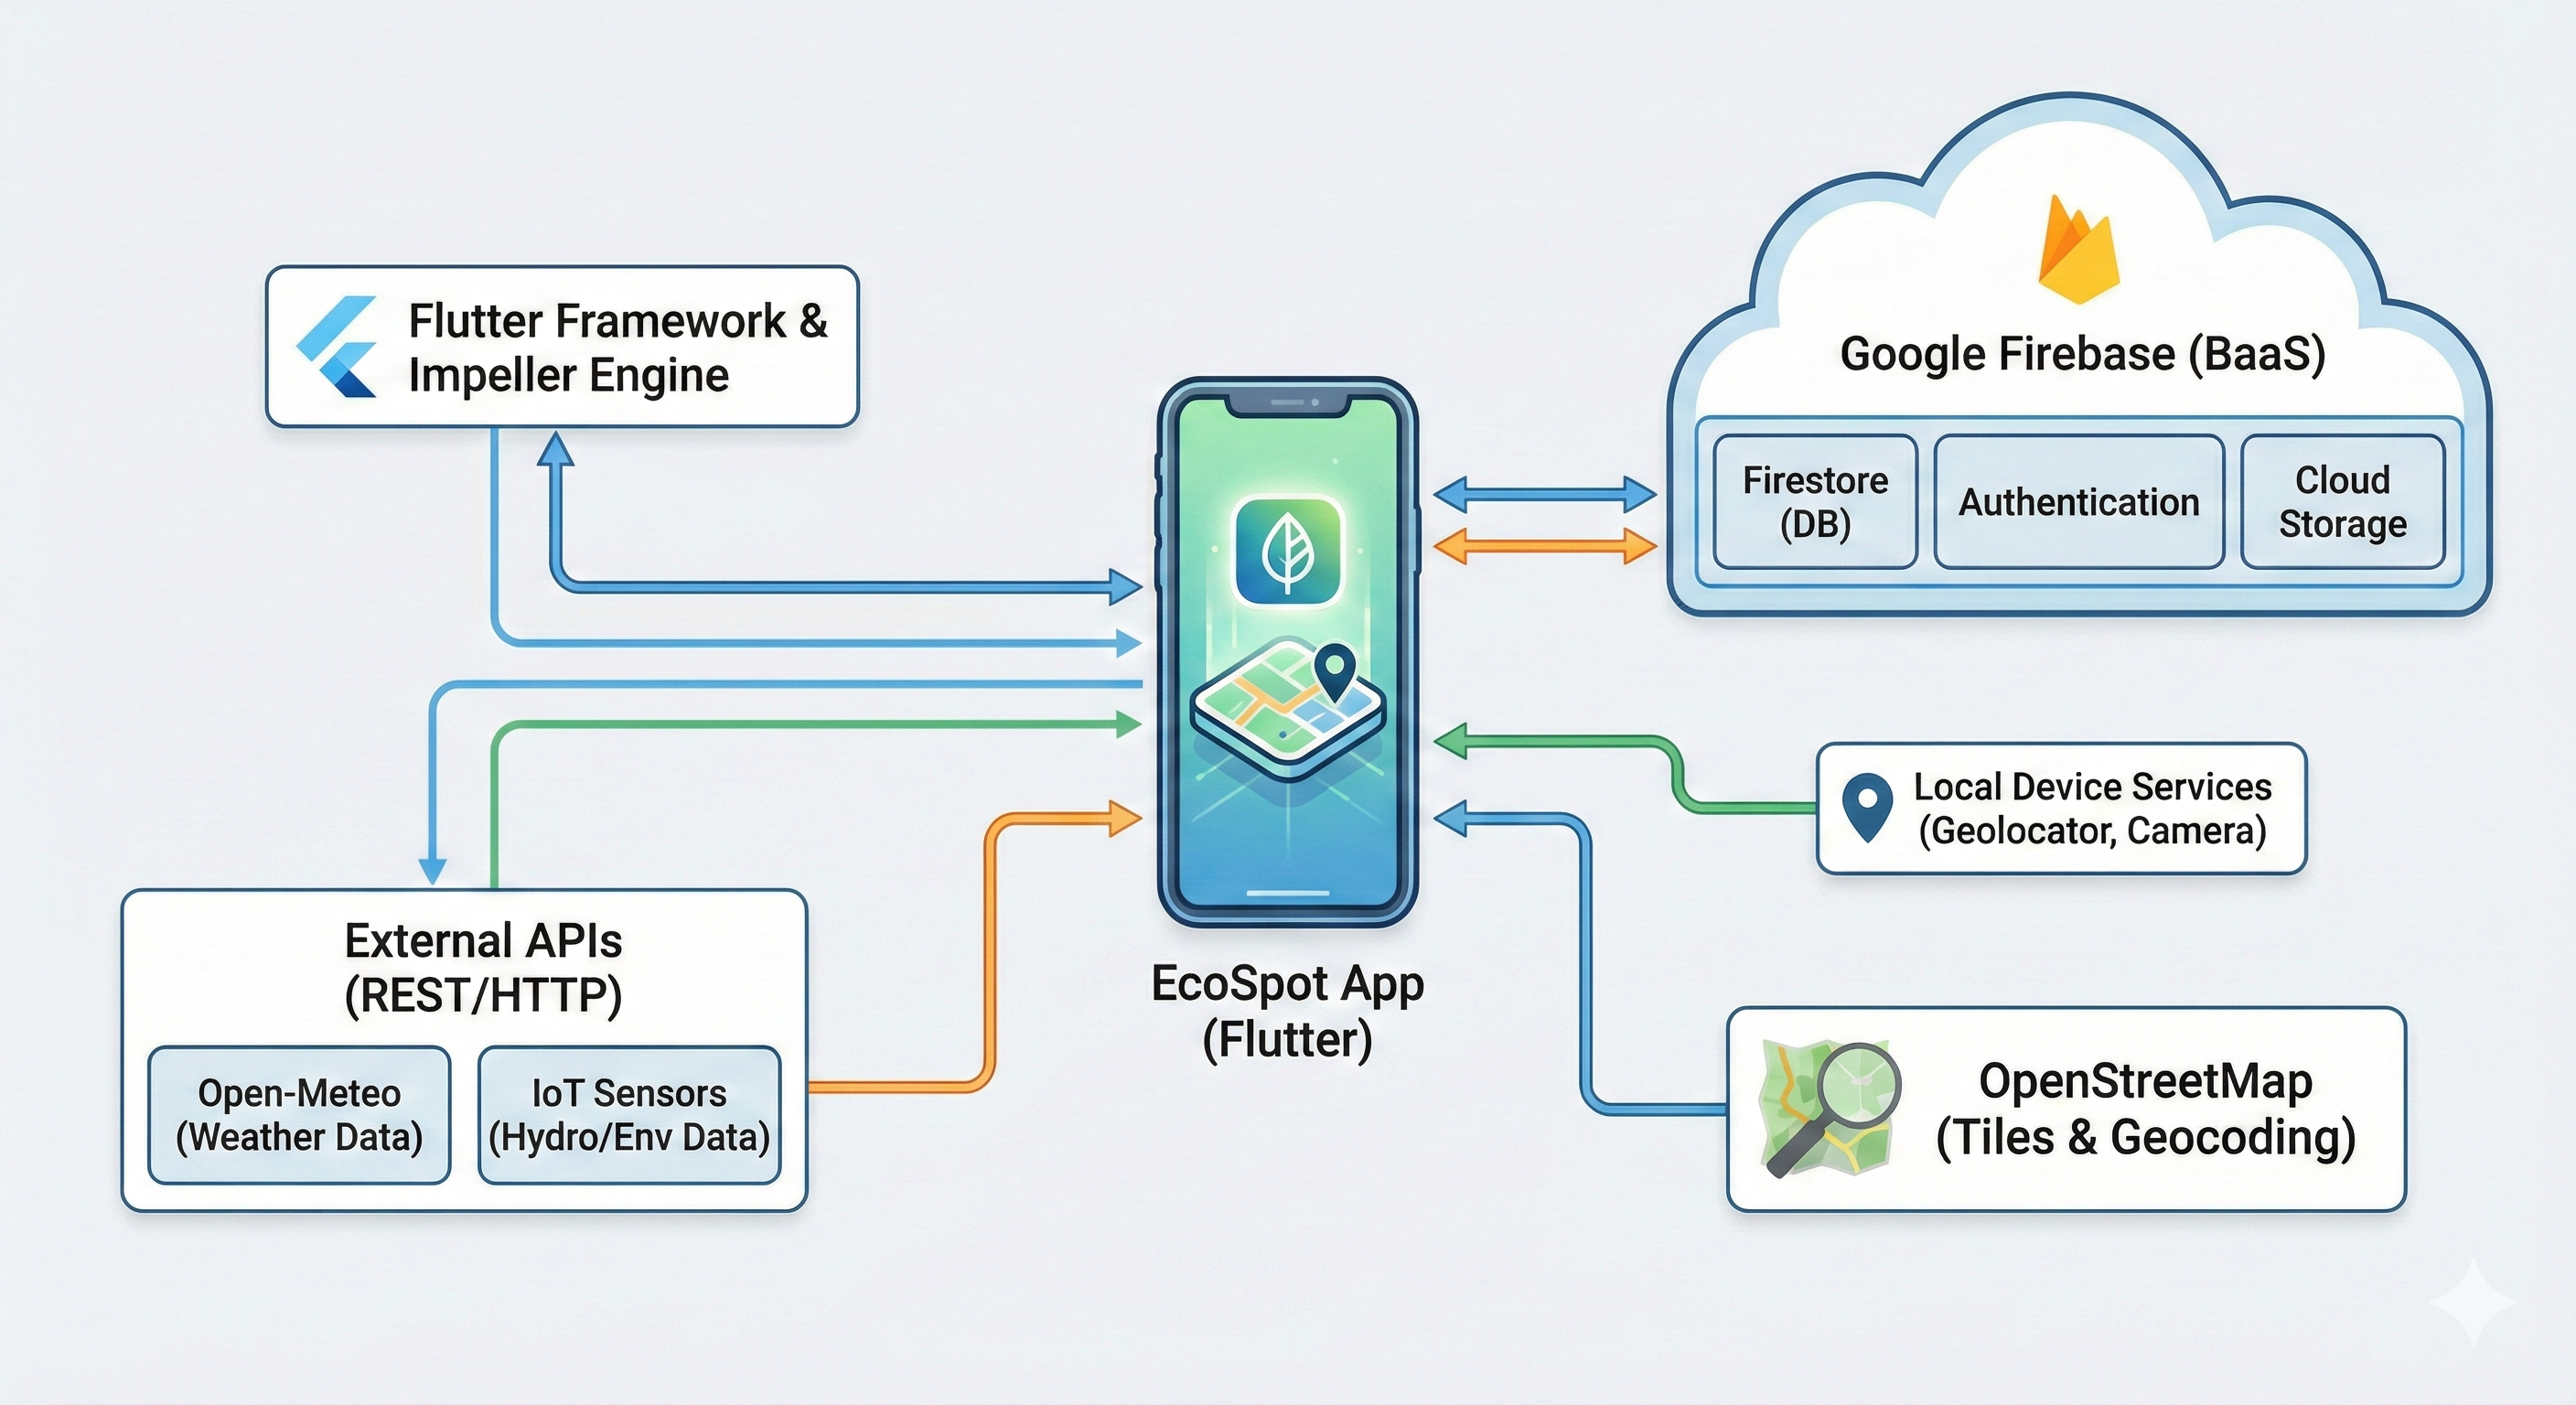
\includegraphics[width=0.9\textwidth]{figures/schema/architecture_schema.png}
    
    \caption[Schema Architetturale di EcoSpot]{Schema logico dell'architettura di sistema.}
    
    \label{fig:system_architecture_schema}
\end{figure}
\section{User Experience}
\label{sec:ux_design}

La progettazione dell'interfaccia utente (UI) di EcoSpot risponde a precise esigenze ergonomiche e comunicative legate al contesto outdoor, adottando le linee guida del \textit{Material Design 3} per garantire coerenza e accessibilità.

\subsection{Palette cromatica}
La palette cromatica di EcoSpot è stata progettata per creare un legame visivo diretto con l'ambiente del Delta del Po e con le iniziative di 
monitoraggio già attive sul territorio. Il colore primario è una tonalità di verde che è stato selezionato ispirandosi all'identità visiva del progetto 
\textit{DISCOV.ER} (Distretti Idro-Socio-Culturali per l'Osservazione e la Valorizzazione delle Risorse) \cite{discover_project}. 

Questa specifica tonalità di verde desaturato è stata scelta per richiamare la vegetazione alofila e le praterie sommerse tipiche delle aree lagunari, con l'obiettivo di trasmettere all'utente un senso di continuità tra l'interfaccia digitale e l'ecosistema circostante. 

Un aspetto centrale della progettazione rimane l'uso semantico del colore per indicare la \textbf{rarità delle specie}, facilitando una valutazione istantanea del valore di un avvistamento sulla mappa:
\begin{itemize}
    \item \textbf{Grigio:} Specie Comuni (\texttt{rarityCommon}).
    \item \textbf{Verde:} Specie Non Comuni (\texttt{rarityUncommon}).
    \item \textbf{Blu:} Specie Rare (\texttt{rarityRare}).
    \item \textbf{Viola:} Specie Epiche (\texttt{rarityEpic}).
    \item \textbf{Oro:} Specie Leggendarie (\texttt{rarityLegendary}).
\end{itemize}
Questa codifica visiva permette all'utente di valutare istantaneamente il valore di una scoperta durante la navigazione sulla mappa.

\subsection{Temi Adattivi}
Per garantire l'usabilità in diverse condizioni ambientali (luce solare diretta o ore crepuscolari), l'applicazione implementa un sistema di \textbf{Temi Adattivi}. Il sistema rileva le preferenze del dispositivo per commutare tra:
\begin{itemize}
    \item \textbf{Light Mode:} Ottimizzato per la leggibilità sotto la luce solare, con sfondi chiari e testi ad alto contrasto.
    \item \textbf{Dark Mode:} Utilizza sfondi scuri per ridurre l'affaticamento visivo e il consumo energetico su dispositivi con schermi OLED, oltre a minimizzare l'impatto luminoso sulla fauna durante le osservazioni serali.
\end{itemize}
L'utente può personalizzare questa impostazione tramite l'area dedicata, con persistenza del dato garantita dalla sincronizzazione sul profilo Firebase.

\subsection{Pattern di Navigazione}
La navigazione è stata progettata per minimizzare il carico cognitivo attraverso una struttura ibrida:
\begin{itemize} 
    \item \textbf{Bottom Navigation Bar:} Costituisce il punto di accesso principale per le macro-aree dell'applicazione (\textit{Esplora}, \textit{Statistiche} e \textit{Impostazioni}), garantendo una transizione rapida tra la mappa e l'area di gestione del profilo. La barra utilizza indicatori visivi e colori semantici per evidenziare la sezione attiva, riducendo lo sforzo mnemonico dell'utente.
    \item \textbf{Modal Bottom Sheets:} Per la visualizzazione dei dettagli di specie, aree verdi e stazioni di monitoraggio, si è scelto di utilizzare dei pannelli a scorrimento che coprono solo parzialmente l'interfaccia. Questa scelta progettuale è fondamentale per preservare il contesto geografico: l'utente può consultare le informazioni descrittive o i dati telemetrici mantenendo visibile la propria posizione sulla mappa in background.
    \item \textbf{Widget di Interazione Rapida:} La mappa integra elementi di controllo posizionati strategicamente per non ostruire la visuale. Sono presenti \textit{Floating Action Buttons} per l'attivazione dei filtri categoriali (layer), per l'invio di segnalazioni di \textit{Citizen Science} e per il ri-centramento della visuale GPS.
    \item \textbf{Sistema di Ricerca e Suggerimenti:} Una barra di ricerca persistente permette di filtrare istantaneamente i contenuti della mappa. Il sistema fornisce suggerimenti dinamici basati sul nome della specie o dell'area verde, facilitando il reperimento di informazioni specifiche anche in presenza di una elevata densità di elementi cartografici.
\end{itemize}

\subsection{Mockup dell'Interfaccia}
\label{subsec:mockups}

Sulla base dei requisiti funzionali e delle linee guida ergonomiche definite, sono stati realizzati i mockup ad alta fedeltà delle schermate principali del sistema. Queste interfacce illustrano la traduzione visiva dell'architettura informativa e dei principi di navigazione ibrida, mostrando come l'utente interagisce con le componenti di esplorazione, gamification e personalizzazione.

Le Figure \ref{fig:mockups_access} e \ref{fig:mockups_management} illustrano il flusso utente principale:

\begin{itemize}
    \item \textbf{Schermata di Accesso:} Costituisce il punto d'ingresso sicuro all'ecosistema EcoSpot. Il design pulito ed essenziale mette in 
    risalto il branding dell'applicazione e offre opzioni chiare per l'autenticazione. È supportato l'accesso ibrido: tramite credenziali proprietarie 
    (email e password) o mediante autenticazione federata (es. Account Google), sfruttando l'integrazione con Firebase Auth per garantire una gestione 
    sicura dell'identità, necessaria per validare le attività di Citizen Science.

   \item \textbf{Home Page:} Rappresenta il fulcro dell'esperienza utente. La mappa interattiva a tutto schermo domina l'interfaccia, 
    massimizzando l'area dedicata all'orientamento spaziale. 
    Per garantire l'immediata identificazione degli elementi cartografici quali Punti di Interesse (POI), fauna locale e aree verdi e la chiara accessibilità 
    delle funzionalità, sono state adottate icone ad alto contrasto che assicurano leggibilità e coerenza stilistica.
    L'interfaccia utilizza un layout a livelli (\textit{overlay}), con elementi flottanti posizionati strategicamente per fornire contesto senza ostruire la visuale: 
    nella parte superiore, la barra di ricerca è affiancata dal widget meteo; 
    lungo il margine destro sono disposti in colonna i \textit{Floating Action Buttons} per le azioni rapide (gestione dei livelli mappa e invio segnalazioni); 
    in basso a destra trova spazio il pulsante per il ricentraggio GPS, mentre alla base l'interfaccia è delimitata dalla 
    \textit{Bottom Navigation Bar} per la navigazione strutturale tra le sezioni.
        
    \item \textbf{Statistiche:} Questa sezione è dedicata al feedback sulla gamification e alla ritenzione dell'utente. 
    Attraverso indicatori visivi chiari (barre di progresso, contatori), l'utente può monitorare il proprio percorso di crescita, visualizzare i punti 
    esperienza (XP) accumulati, il rango attuale e la distanza dall'obiettivo successivo. La schermata funge anche da 
    registro storico delle specie scoperte, rinforzando il senso di realizzazione.

    \item \textbf{Impostazioni:} Offre all'utente il controllo sull'esperienza d'uso. Oltre alla gestione del profilo e alla disconnessione sicura, questa 
    schermata ospita i controlli di accessibilità e preferenza visiva. In particolare, il selettore per il Tema Adattivo (chiaro/scuro) permette di adeguare 
    l'interfaccia alle condizioni di luminosità ambientale, garantendo la leggibilità sia sotto il sole diretto che durante le osservazioni crepuscolari.
\end{itemize}

\begin{figure}[H]
    \centering
    \begin{subfigure}[b]{0.30\textwidth}
        \centering
        \includegraphics[width=\textwidth]{figures/mockups/login.png} 
        \caption{Schermata di Login}
        \label{fig:login_mockup}
    \end{subfigure}
    \hfill
    \begin{subfigure}[b]{0.30\textwidth}
        \centering
        \includegraphics[width=\textwidth]{figures/mockups/home.png} 
        \caption{Home Page}
        \label{fig:home_mockup}
    \end{subfigure}
    \caption{Mockup delle schermate di accesso e navigazione principale. Nella Home Page, le icone utilizzate per i marker e l'interfaccia provengono 
    dalla libreria Icons8.}
    \label{fig:mockups_access}
\end{figure}

\begin{figure}[H]
    \centering
    \begin{subfigure}[b]{0.30\textwidth}
        \centering
        \includegraphics[width=\textwidth]{figures/mockups/statistiche.png} 
        \caption{Schermata Statistiche}
        \label{fig:stats_mockup}
    \end{subfigure}
    \hfill
    \begin{subfigure}[b]{0.30\textwidth}
        \centering
        \includegraphics[width=\textwidth]{figures/mockups/impostazioni.png} 
        \caption{Schermata Impostazioni}
        \label{fig:settings_mockup}
    \end{subfigure}
    \caption{Mockup delle schermate di progressiGeograficane utente (Statistiche) e configurazione dell'interfaccia (Impostazioni).}
    \label{fig:mockups_management}
\end{figure}
\section{Modellazione e Progettazione dei Dati}
\label{sec:data_modeling}

La traduzione dei requisiti informativi in una struttura dati coerente ha richiesto la progettazione di classi di dominio specifiche, atte a gestire la complessità delle interazioni spaziali e della progressione dell'utente. Il sistema adotta un paradigma NoSQL orientato ai documenti tramite \textit{Google Cloud Firestore}, ottimizzando le performance di lettura e la sincronizzazione in tempo reale.

\subsection{Architettura del Database: Cloud Firestore}
Per soddisfare i requisiti di scalabilità e sincronizzazione real-time, è stato scelto un database NoSQL organizzato in \textbf{Collezioni} di \textbf{Documenti} JSON-like. Questa scelta progettuale offre vantaggi specifici per il contesto di EcoSpot:
\begin{itemize}
    \item \textbf{Struttura Gerarchica:} Permette di incapsulare dati complessi, come la lista delle specie sbloccate, direttamente nel documento utente, migliorando la reattività dell'app.
    \item \textbf{Aggiornamenti in Tempo Reale:} Grazie ai listener nativi, qualsiasi modifica critica (es. aumento di livello) viene propagata istantaneamente all'interfaccia senza refresh manuale.
    \item \textbf{Funzionamento Offline:} Il database mantiene una cache locale, permettendo la consultazione dei dati anche in zone del Parco del Delta del Po prive di copertura di rete.
\end{itemize}

\subsection{Entità del Dominio}
La modellazione del database riflette le classi definite nel dominio applicativo, strutturate per supportare le funzionalità di gamification e monitoraggio:

\begin{itemize}
    \item \textbf{Utente:} Memorizza lo stato dinamico della progressione, inclusi i punti esperienza (XP) e il registro delle scoperte 
    (\texttt{visitedSpeciesIds}). La logica associata determina dinamicamente il \textit{rango} dell'utente (da "Esploratore" a "Leggenda del Delta") 
    tramite estensioni dedicate.
    
    \item \textbf{Habitat e Aree Verdi:} Unifica fauna e flora in un modello che integra metadati e parametri geospaziali. Ogni specie definisce un raggio di 
    scoperta (\texttt{discoveryRadius}) 450 metri per gli animali e 800 metri per le aree verdi per adattare il \textit{geofencing} alla natura dell'entità.
    
    \item \textbf{Punti di Interesse e API:} Modella le stazioni \ac{IoT} e i punti di interesse. La struttura è popolata tramite polling asincrono che mappa 
    ID sensore eterogenei a parametri fisici leggibili come temperatura, livello idrometrico e conducibilità.
    
    \item \textbf{Segnalazioni:} Gestisce i contributi di Citizen Science, associando i metadati dell'utente a coordinate GPS precise  
    e riferimenti a risorse multimediali archiviate su \textit{Cloud Storage}.
\end{itemize}

\subsection{Logica di Integrazione e Gamification}
La progettazione prevede un livello di servizi dedicato all'orchestrazione dei dati:

\begin{itemize}
    \item \textbf{Valore Atteso della Progressione:} Il progresso verso il livello successivo è calcolato come il rapporto tra gli XP attuali e la soglia di 1000 XP per livello. Tale parametro rappresenta il \textbf{Valore Atteso} della crescita ed è visualizzato tramite indicatori lineari nella pagina delle statistiche.
    
    \item \textbf{Integrità delle Scoperte:} Per garantire la coerenza, il sistema utilizza transazioni atomiche durante la fase di scoperta. Ciò assicura che l'incremento di esperienza e la registrazione della specie avvengano come un'unica operazione indivisibile.
    
    \item \textbf{Contestualizzazione Ambientale:} L'integrazione con le API di \textit{Open-Meteo} arricchisce i POI con informazioni atmosferiche locali, calcolate dinamicamente in base alle coordinate geografiche dello stesso.
\end{itemize}

\subsection{Relazioni e Considerazioni Progettuali}
Nel paradigma NoSQL, le relazioni privilegiano la performance di lettura rispetto alla normalizzazione:
\begin{itemize}
    \item \textbf{Relazione Utente-Specie (M:N):} Implementata salvando un array di identificatori direttamente nel documento utente per ridurre la necessità di \textit{join} costose.
    \item \textbf{Relazione Utente-Segnalazioni (1:N):} Le segnalazioni mantengono un riferimento all'identificativo utente (\texttt{userId}), permettendo query indicizzate per visualizzare lo storico personale.
    \item \textbf{Estensibilità:} Il modello permette l'aggiunta di nuove entità senza richiedere migrazioni rigide dello schema, garantendo un'evoluzione continua del sistema.
\end{itemize} 
\chapter{Sviluppo e Implementazione}
\label{chap:implementation}

Questo capitolo descrive le fasi realizzative dell'applicazione \textit{EcoSpot}, analizzando l'architettura del software, le scelte tecniche per lo sviluppo mobile e l'implementazione delle funzionalità core come la mappa interattiva, il sistema di gamification e l'integrazione dei sensori IoT.

\section{Architettura del Progetto}
Il progetto è stato strutturato seguendo una divisione in layer logici per garantire manutenibilità e scalabilità del codice. La cartella sorgente (\texttt{lib}) è organizzata nei seguenti moduli principali:

\begin{itemize}
    \item \textbf{Data Layer}: Contiene le definizioni delle entità (es. \texttt{UserModel}, \texttt{Species}, \texttt{SensorData}) e la logica di persistenza dei dati.
    \item \textbf{Service Layer}: Gestisce la comunicazione con i servizi esterni. Qui risiedono \texttt{AuthService} per l'autenticazione, \texttt{SensorService} per i dati IoT e \texttt{WeatherService} per le API meteo.
    \item \textbf{Presentation Layer}: Comprende i widget dell'interfaccia utente (\texttt{pages} e \texttt{widgets}), separando la logica di visualizzazione dallo stato dell'applicazione.
\end{itemize}

\subsection{Sincronizzazione dati}
L'implementazione della logica reattiva si basa sull'utilizzo degli \texttt{StreamProvider} di Riverpod. Nel caso del tracciamento utente, il provider \texttt{userPositionProvider} sottoscrive lo stream di eventi del plugin Geolocator. Come mostrato nella sezione successiva, il widget \texttt{MapWidget} consuma questo stato: ogni volta che il GPS rileva un movimento, il provider emette un nuovo oggetto \texttt{Position}, causando il rebuild parziale della sola componente mappa senza intaccare il resto dell'interfaccia, ottimizzando così le risorse del dispositivo mobile.

\section{Sviluppo dell'Applicazione Mobile}
Lo sviluppo si è concentrato sulla creazione di un'esperienza utente fluida, sfruttando le capacità multi-piattaforma di Flutter.

\subsection{Mappa Interattiva e Clustering}
La visualizzazione cartografica è il punto centrale dell'interazione ed è gestita dal widget \texttt{MapWidget}, che integra la libreria \texttt{flutter\_map} \cite{fluttermap}. 

Per gestire l'elevato numero di marker (animali, piante, sensori) senza compromettere le prestazioni di rendering, è stato implementato un sistema di clustering tramite il pacchetto \texttt{flutter\_map\_marker\_cluster}. Questo permette di raggruppare visivamente i punti di interesse vicini in un unico indicatore numerico quando lo zoom della mappa è basso, espandendosi automaticamente quando l'utente ingrandisce la visuale.

Il codice \ref{lst:map_markers} mostra come vengono renderizzati i marker per le aree verdi utilizzando i widget nativi di Flutter:

\begin{listing}[H]
\begin{minted}[frame=single, breaklines]{dart}
// Rendering dei marker sulla mappa (estratto da MapWidget)
...widget.greenAreas.map((area) {
  return Marker(
    point: area.centerPoint,
    width: 70,
    height: 70,
    child: GestureDetector(
      onTap: () {
        showModalBottomSheet(
          context: context,
          builder: (context) => GreenAreaDetailSheet(species: area),
        );
      },
      child: Image.asset(area.imagePath),
    ),
  );
})
\end{minted}
\caption{Rendering dei marker interattivi sulla mappa}
\label{lst:map_markers}
\end{listing}

\subsection{Gestione Gamification}
Il cuore dell'esperienza utente è il sistema di scoperta ("Discovery"), progettato per incentivare l'esplorazione fisica del Parco. L'app calcola costantemente la distanza geodetica tra la posizione dell'utente e quella delle specie target.

\subsubsection{Logica di Scoperta}
Quando la distanza rilevata è inferiore al parametro \texttt{discoveryRadius}, viene invocato il metodo di scoperta. L'algoritmo (Listing \ref{lst:discovery}) è implementato sfruttando la precisione del GPS del dispositivo mobile per validare la presenza dell'utente in loco.

\begin{listing}[H]
  \begin{minted}[frame=single, breaklines]{dart}
void _checkDiscoveries(LatLng userLocation) {
  // Calcolo distanza geodetica
  final double meters = _distanceCalculator.as(
      LengthUnit.Meter, userLocation, species.centerPoint);

  // Verifica soglia di scoperta
  if (meters <= species.discoveryRadius) {
    _triggerDiscovery(user.uid, species);
  }
}
  \end{minted}
  \caption{Algoritmo di scoperta basato sulla distanza geodetica}
  \label{lst:discovery}
\end{listing}

\subsubsection{Utente e Rango}
Il modello utente (\texttt{UserModel}) calcola dinamicamente il livello e il rango (es. "Guardiano", "Leggenda") in base ai punti esperienza (XP) accumulati con le scoperte. Questo aggiornamento avviene in tempo reale, sbloccando nuovi badge visibili nella sezione profilo.

\subsubsection{Segnalazioni}
Gli utenti possono contribuire attivamente al monitoraggio ambientale tramite la funzione di segnalazione. Il widget \texttt{ReportDialog} permette di acquisire una fotografia, associare automaticamente le coordinate GPS attuali e inserire una descrizione dell'avvistamento. Questi dati vengono incapsulati in un oggetto \texttt{ReportModel} e inviati a Firestore per la validazione e la storicizzazione.

\subsection{Integrazione Sensori}
Per fornire un quadro dello stato ambientale del Parco, l'applicazione integra dati provenienti da stazioni di monitoraggio reali. Il servizio \texttt{SensorService} interroga l'API esterna ed effettua il parsing dei dati JSON ricevuti dalle stazioni (es. Bellocchio, Foce).

\begin{listing}[H]
  \begin{minted}[frame=single, breaklines]{dart}
final response = await http.post(Uri.parse(_apiUrl), ...);

if (response.statusCode == 200) {
  final decodedBody = jsonDecode(response.body);
  // Estrazione e normalizzazione valore sensore
  value = decodedBody['sensorValue'] ?? decodedBody['value'];
  return MapEntry(sensorName, value ?? "N/D");
}
  \end{minted}
  \caption{Parsing dei dati JSON dai sensori IoT}
  \label{lst:sensor_parsing}
\end{listing}

Questi dati vengono presentati all'utente tramite popup informativi accessibili cliccando sulle icone delle stazioni sulla mappa, fornendo parametri aggiornati come temperatura, livello idrometrico e conduttività.

\section{Interfaccia Utente}
L'interfaccia è stata costruita rispettando le linee guida del Material Design 3. Le viste principali includono:

\begin{itemize}
    \item \textbf{Home Dashboard}: Una panoramica che sovrappone alla mappa il meteo locale (tramite \texttt{WeatherService}) e i controlli di navigazione.
    \item \textbf{Schede di Dettaglio}: Implementate tramite \texttt{DraggableScrollableSheet}, queste viste modali (es. \texttt{SpeciesDetailSheet}) forniscono informazioni educative e multimediali mantenendo visibile il contesto geografico sottostante.
    \item \textbf{Profilo e Statistiche}: Una sezione dedicata alla visualizzazione delle specie collezionate e del rango raggiunto, con grafici di progresso.
\end{itemize}

\section{Gestione dello Stato}
La gestione globale dello stato è affidata al file \texttt{app\_providers.dart}, che definisce i provider Riverpod per l'intera applicazione. Questo approccio centralizzato permette di iniettare le dipendenze (come \texttt{DatabaseHelper} o \texttt{AuthService}) in qualsiasi widget senza passare parametri esplicitamente, garantendo che l'interfaccia reagisca istantaneamente ai cambiamenti dei dati sottostanti.

% 4. Conclusioni
% \unchapter{Conclusioni}

Lorem ipsum dolor sit amet consectetur adipisicing elit. Esse illo, nulla quo laboriosam eaque aperiam dolore excepturi voluptates fuga magnam dolores quis, nobis blanditiis, voluptas impedit beatae tempora porro aliquid mollitia eveniet quos quae. Incidunt doloremque, quo quaerat totam voluptate accusantium, deleniti consequuntur ullam, sequi sunt perferendis repudiandae. Suscipit assumenda reprehenderit quibusdam voluptate, alias expedita molestias, beatae numquam totam deserunt quidem fugit quas nulla omnis molestiae fugiat nostrum! Quam, quisquam consequuntur velit consequatur nesciunt doloribus dolorum exercitationem. At, atque harum. Dolorum, ut! Quod similique deserunt explicabo illum, odio consequatur quibusdam id dolorum sint eum pariatur saepe asperiores doloremque aliquid sequi praesentium harum, molestias minus quaerat. Provident modi facere repellendus eius et quae deserunt ex molestias iure, dignissimos est autem, accusantium tenetur voluptas quos maiores ullam quisquam a laudantium qui inventore asperiores tempora.

% 5. Bibliografia
\cleardoublepage
\addcontentsline{toc}{chapter}{Bibliografia}
\nocite{*}
\bibliography{bibliography} % Legge il file bibliography.bib

% 6. Ringraziamenti
\unchapter{Ringraziamenti}

\thispagestyle{empty}

Giunto al termine di questo percorso accademico, desidero ringraziare tutti coloro che 
hanno contribuito, in modi diversi, al raggiungimento di questo traguardo.

In questo percorso ho conosciuto tante persone, tra cui Lorenzo, che desidero 
ringraziare personalmente per il suo supporto e la sua presenza. Un pensiero speciale va 
anche ai miei amici di sempre e a quelli conosciuti lungo il cammino, per i momenti di svago, 
i confronti accesi e per aver reso più leggeri anche i periodi di studio più intensi. 
Senza le nostre pause e il supporto reciproco, questo cammino sarebbe stato certamente più faticoso.

Voglio ringraziare in modo particolare Enrico, che mi ha dato una spinta, anche più di una, 
per entrare in questo mondo nel quale, probabilmente, non ci sarei mai entrato da solo.

Infine, il ringraziamento più grande va alla mia famiglia: ai miei genitori e a mia sorella, 
per aver sempre creduto in me e per avermi sostenuto in ogni scelta. Grazie per avermi 
dato la forza e la possibilità di arrivare fin qui.

A tutti voi, grazie.



\end{document}